\documentclass[english]{article}
\renewcommand{\thesection}{\arabic{section}} % Redefine section numbering format
\usepackage[english]{babel} 
\usepackage[T1]{fontenc}
\usepackage[utf8x]{inputenc}
\usepackage{float}
\usepackage{graphicx}
\usepackage{svg}
\usepackage{siunitx}
\makeatletter
\usepackage[a4paper,top=2cm,bottom=2cm,left=2cm,right=2cm]{geometry}
\usepackage{enumitem}
\usepackage{subfig}
\usepackage{amsthm}
\usepackage{amsmath}
\usepackage{epstopdf}
\usepackage{fancyhdr}
\usepackage{booktabs,array}

\hyphenation{english}
\makeatother

\usepackage{babel}


\usepackage{listings}
\usepackage{xcolor} % for setting colors

% set the default code style
\lstset{
    frame=tb, % draw a frame at the top and bottom of the code block
    tabsize=4, % tab space width
    showstringspaces=false, % don't mark spaces in strings
    numbers=left, % display line numbers on the left
    commentstyle=\color{gray}, % comment color
    keywordstyle=\color{blue}, % keyword color
    stringstyle=\color{red} % string color
}

\begin{document}
\setcounter{section}{-1} % Set section counter to -1
\begin{titlepage}

	\begin{center}
		\begin{Large} \textbf{UNIVERSITY OF PADOVA} \\
		\end{Large} \vspace{1cm}
		\vspace{3cm}
		\begin{Large} Embedded Real--Time Control \end{Large}
		\par\end{center}

	\begin{center}
		\begin{Large}Laboratory report\\
		\end{Large}
		\par\end{center}

	\begin{center}
		\vspace{2cm}
		\begin{figure}[!htb]
			\centering 
\includegraphics[width=8cm]{figures/unipd-logo.png}\\

		\end{figure}

		\par\end{center}

	\begin{center}
		\vspace{2cm}
		\begin{Large} 
                Maximilian Kloevekorn-Fischer - (2096189) \\
                Mohammadjavad Rajabi - (2085121) \\
                Pouria Zakariapour - (2072836) \\
                Parsa Majidi - (2080216)  \\
		\end{Large} \vspace{2cm}
		\begin{Large} Academic Year 2022-2023 \end{Large}
		\par\end{center}

\end{titlepage}

\tableofcontents
\newpage
\section{Abstract}
During this course the mobile robotics platform equipped with motors, sensors, interfaces, and different processing units was the case of study. In the following report it will be referenced as TurtleBot shown in Figure \ref{fig:turtlebot}. The main processing unit is the STM32F767 microcontroller, it is connected directly or indirectly to all inputs and outputs via GPIOs.
\begin{figure}[!h]
	\centering
	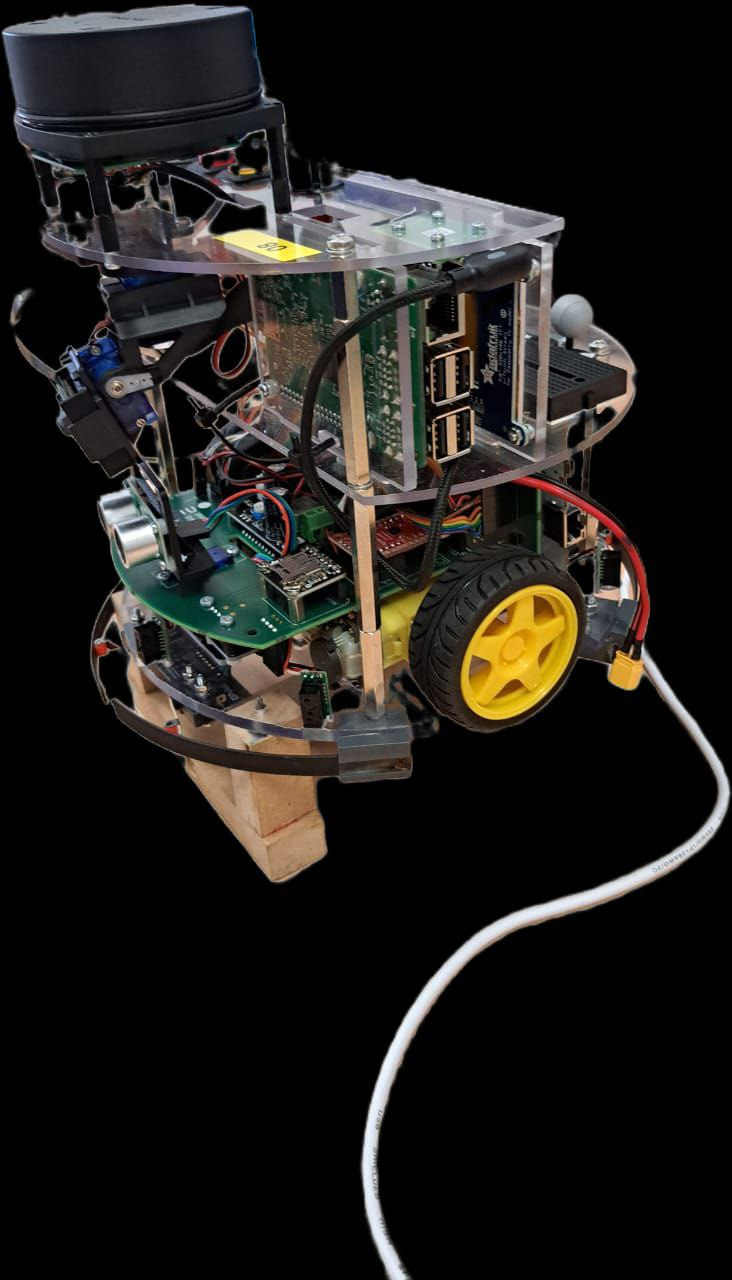
\includegraphics[width=0.4\textwidth]{figures/turtlebot.jpg}
	\caption{The TurtleBot}
	\label{fig:turtlebot}
\end{figure}

\newpage
\section{Laboratory 1: I2C}
The purpose of this lab can be categorized as follows:
\begin{itemize}
    \item Inter-Integrated Circuit (I2C)
    \item SX1509 I/O Expander
    \item APIs
\end{itemize}

\subsection{Description}
This laboratory aims to explore and gain practical experience with some fundamental concepts in Embedded Systems.
 In particular, the focus is working with the I2C protocol and the SX1509 module, as well as understanding 
and utilizing interrupts in the STM32F767 microcontroller. Throughout this laboratory, we will delve into several exercises that will provide us with hands-on experience in applying these concepts.

\subsubsection{Inter-Integrated Circuit (I2C)}
The I2C bus is a standard bidirectional interface that uses a controller, known as
the master, to communicate with slave devices, Shown in Figure \ref{fig:I2C}. 
\begin{figure}[!h]
	\centering
	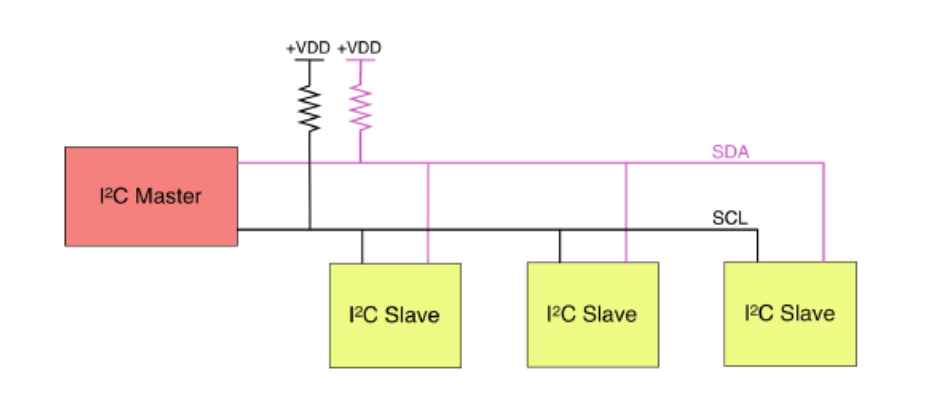
\includegraphics[width=0.65\textwidth,]{figures/I2C_Connection.png}
	\caption{I2C Connection Scheme}
	\label{fig:I2C}
\end{figure}

A slave may not transmit data unless it has been addressed by the master. 
Each device on the I2C bus has a specific device address to differentiate between
other devices that are on the same I2C bus. Many slave devices will require configuration upon startup to set the behavior of
the device. This is typically done when the master accesses the slave's internal
register maps, which have unique register addresses. A device can have one or
multiple registers where data is stored, written, or read. The physical I2C interface consists of the serial clock (SCL) and serial data (SDA) lines. 
Both SDA and SCL lines must be connected to VCC through a pull-up resistor. The size
of the pull-up resistor is determined by the amount of capacitance on the I2C lines.
Shown in Figure (\ref{fig:pulling}) and Figure (\ref{fig:releasing})
\begin{figure}[!ht]
	\centering
	\subfloat[Pulling the Bus Low with an open-drain Interface ]
	{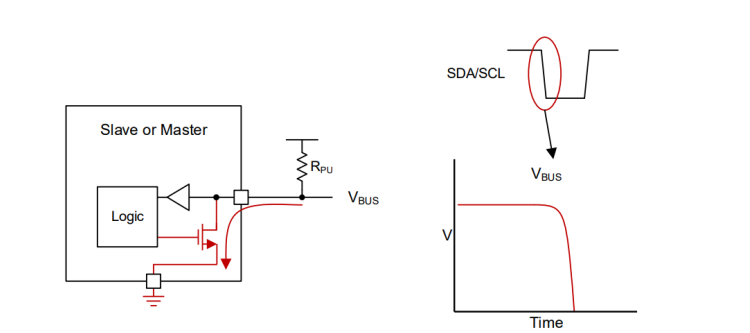
\includegraphics[width=0.45\textwidth,height=0.25\textwidth]{figures/Pulling-the-bus.png}
		\label{fig:pulling}}
	\subfloat[Releasing the bus with an open-drain interface]
	{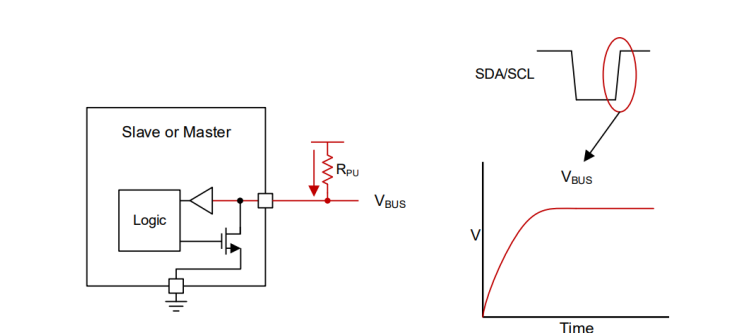
\includegraphics[width=0.45\textwidth,height=0.25\textwidth]{figures/Releasing-the-bus.png}
		\label{fig:releasing}}
	\caption{}
\end{figure}
\newpage
The protocol transmits messages composed by a 9 bit packet. Each message begins with
 the µC generation of a start signal and ends with a stop signal from the microcontroller,
 Shown in Figure \ref{fig:Stop}.
 \begin{figure}[!h]
	\centering
	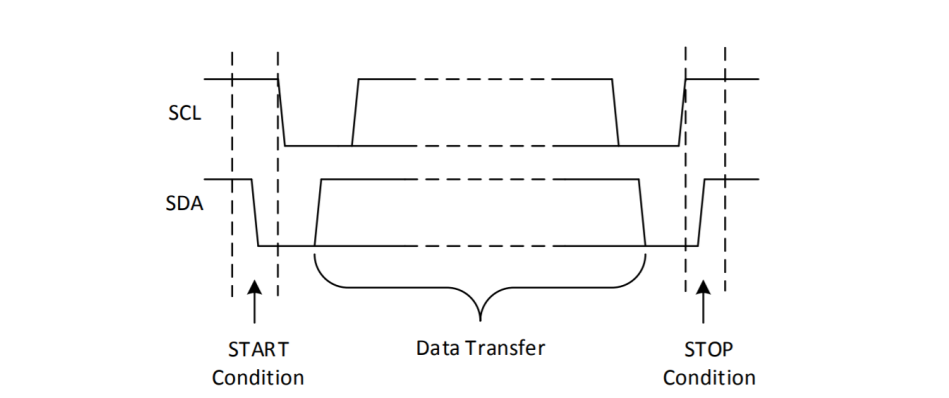
\includegraphics[width=0.80\textwidth,]{figures/Start-Stop.png}
	\caption{Example of Start and Stop condition}
	\label{fig:Stop}
\end{figure}

The start and stop conditions are characterized by the data line that
moves towards low (start) or high (stop) during the clock high phase.
Any other bit is set during the low clock phase. This ensures that the
start and stop condition can be discriminated from any other data
transmission.\newline

In this communication protocol, each packet consists of 9 bits. 
The first 8 bits are transmitted by the sending unit, while the 9th bit is set by the receiving unit. 
The order of the bits within each byte follows a "Most Significant Bit" (MSB) format. 
The 9th bit serves as an reply, indicating whether the receiver acknowledges the data. 
To acknowledge, the receiver sets the data line to a low state at the 9th bit position.
Example of Single Byte data transfer in Figure \ref{fig:Data}.
\begin{figure}[!h]
	\centering
	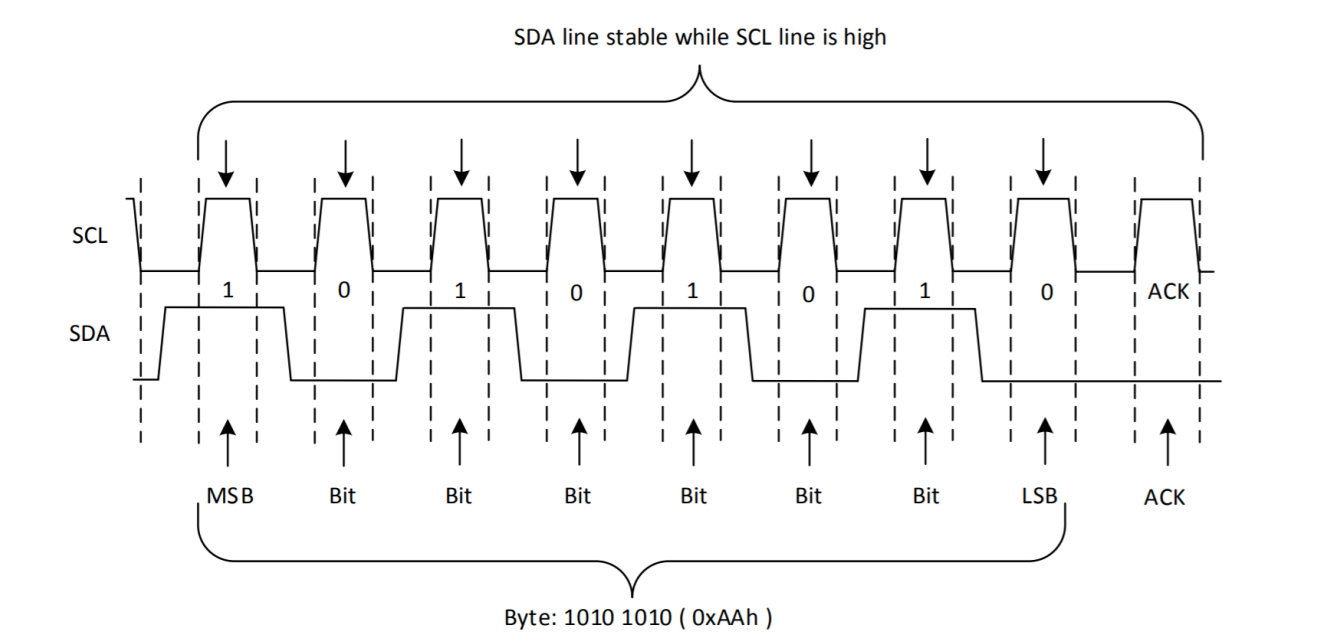
\includegraphics[width=0.80\textwidth,]{figures/Single_byte.png}
	\caption{Example of Single Byte Data Transfer}
	\label{fig:Data}
\end{figure}

\subsubsection{SX1509 I/O Expander}
The SX1509 is a general purpose GPIO expander board, able to parallel handle several inputs and outputs. It has ultra-low voltage capabilities of 1.2 to 3.6 V, ideal for battery powered equipment. This family of
GPIOs comes in 4-, 8-, 16-channel configuration and
allows easy serial expansion of I/O through a
standard 400kHz I2C interface. GPIO devices can
provide additional control and monitoring when the
microcontroller or chipset has insufficient I/O ports, or
in systems where serial communication and control
from a remote location is advantageous. Keypad application is also supported with
the on-chip scanning engine. It enables
continuous keypad monitoring up to 64 keys without
any additional host interaction, keeping the bus activity low. The SX1509 has the ability to generate mask-programmable interrupts based on
falling/rising edge of any of its GPIO lines. \newline

In this setup, two SX1509 modules are connected to the microcontroller using the I2C bus. 
Both devices share the same I2C line, specifically I2C1. To differentiate between the two modules,
we assign a specific slave address to each. 
The first SX1509, referred to as sx1509\_1, is assigned
  the slave address 0x3E, while the second module, known as sx1509\_2, is associated with the slave address 0x3F.
\\Allocated addresses of slaves implemented in Listing \ref{lst:addr}
\begin{lstlisting}[language=C, caption={I2C Addresses}, label={lst:addr} ]
#define SX1509_I2C_ADDR1 0x3E       //SX1509 Proxy Sensors I2C address
#define SX1509_I2C_ADDR2 0x3F       //SX1509 Keypad I2C address
\end{lstlisting}
The two lines of Listing \ref{lst:add} are addressing of SX1509 registes for Keypad.
\begin{lstlisting}[language=C, caption={Keypad Data registers}, label={lst:add} ]
#define REG_KEY_DATA_1  0x27        //RegKeyData1 Key value (column) 1111 1111
#define REG_KEY_DATA_2  0x28	    //RegKeyData2 Key value (row) 1111 1111
\end{lstlisting}
This addressing scheme allows the microcontroller to communicate with each SX1509 module individually over the shared I2C bus,
Figure \ref{fig:SX1509}
\begin{figure}[!h]
	\centering
	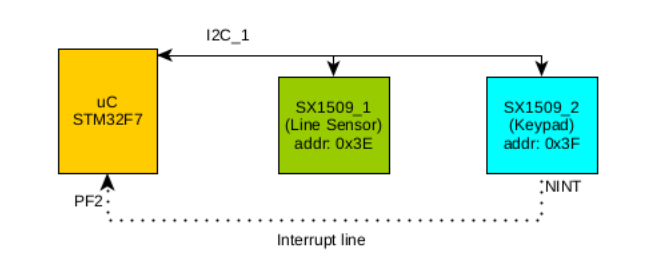
\includegraphics[width=0.80\textwidth,]{figures/SX.png}
	\caption{SX1509 connected to Keypad and Line sensor}
	\label{fig:SX1509}
\end{figure}
\subsubsection{APIs}
The HAL (Hardware Abstraction Layer) API (Application Programming Interface) 
is a software layer provided by STM32 microcontrollers that abstracts
 the underlying hardware functionalities and provides a standardized 
 interface for developers to interact with the microcontroller's peripherals and features.
The HAL API serves as a bridge between the application software and the hardware, 
allowing developers to access and control the microcontroller's peripherals,
such as GPIO (General Purpose Input/Output), UART (Universal Asynchronous Receiver-Transmitter),
SPI (Serial Peripheral Interface), I2C (Inter-Integrated Circuit), 
timers, and more. It provides a higher-level programming interface,
hiding the low-level hardware details and offering a set of functions that
encapsulate complex hardware operations. \newline
Listing \ref{lst:read} are useful HAL functions that we used during this Laboratory.
\begin{lstlisting}[language=C, caption={Reading Register values}, label={lst:read} ]
HAL_StatusTypeDef HAL_I2C_Mem_Read(I2C_HandleTypeDef *hi2c, uint16_t
    DevAddress, uint16_t MemAddress, uint16_t MemAddSize, uint8_t *pData,
    uint16_t Size, uint32_t Timeout);
\end{lstlisting}
Read an amount of data in blocking mode from a specific memory address  
\begin{itemize}
    \item \textbf{hi2c} Pointer to a I2C\_HandleTypeDef structure that contains the configuration information
    for the specified I2C.
    \item \textbf{DevAddress} Target device address: The device 7 bits address value in datasheet must be
    shifted to the left before calling the interface.
    \item \textbf{MemAddress} Internal memory address
    \item \textbf{MemAddSize} Size of internal memory address
    \item \textbf{pData} Pointer to data buffer
    \item \textbf{Size} Amount of data to be sent
    \item \textbf{Timeout} Timeout duration
    \item \textbf{return value} HAL status
\end{itemize}

\begin{lstlisting}[language=C, caption={Writing Register values}, label={lst:write} ]
HAL_StatusTypeDef HAL_I2C_Mem_Write(I2C_HandleTypeDef *hi2c, uint16_t
    DevAddress, uint16_t MemAddress, uint16_t MemAddSize, uint8_t *pData,
    uint16_t Size, uint32_t Timeout)
\end{lstlisting}
Write an amount of data in blocking mode to a specific memory address
\begin{itemize}
    \item \textbf{hi2c} Pointer to a I2C\_HandleTypeDef structure that contains the configuration information
        for the specified I2C.
        \item \textbf{DevAddress} Target device address: The device 7 bits address value in datasheet must be
        shifted to the left before calling the interface.
        \item \textbf{MemAddress} Internal memory address
        \item \textbf{MemAddSize} Size of internal memory address
        \item \textbf{pData} Pointer to data buffer
        \item \textbf{Size} Amount of data to be sent
        \item \textbf{Timeout} Timeout duration 
        \item \textbf{return value} HAL status
\end{itemize}

\newpage
\subsection{Exercises}
\subsubsection{Exercise 1:}
In this exercise we are asked to write an ISR that recognize and correctly handles the keypad interrupts. We properly implemented the void HAL\_GPIO\_EXTI\_Callback(uint16\_t pin) function, which is used in conjunction with the EXTI (External Interrupt) peripheral to handle interrupts generated by GPIO pins. Then the triggered interrupt is printed i.e. the pin. To be able to receive another interrupt from the keypad, we read
the registers REG\_KEY\_DATA\_1 and REG\_KEY\_DATA\_2 inside the ISR.
\begin{lstlisting}[language=C, caption={Interrupt Callback}]
void HAL_GPIO_EXTI_Callback(uint16_t GPIO_Pin){
    /*Reading Data From SX1509_I2C_ADDR2 Device Address and REG_KEY_DATA_1 and 
    REG_KEY_DATA_2 Memory Addresses */
    HAL_StatusTypeDef status;
    status = HAL_I2C_Mem_Read(
        &hi2c1,
        SX1509_I2C_ADDR2 << 1,
        REG_KEY_DATA_1,
        1,
        &colum,
        1,
        I2C_TIMEOUT
    );
    if (status != HAL_OK) {
        printf("Error occurred during reading I2C, REG_KEY_DATA_1\n");
    }
    status = HAL_I2C_Mem_Read(
        &hi2c1,
        SX1509_I2C_ADDR2 << 1,
        REG_KEY_DATA_2, 1,&row,
        1, 
        I2C_TIMEOUT
    );
    if (status != HAL_OK) {
        printf("Error occurred during reading I2C, REG_KEY_DATA_2\n");
    }
    printf("Interrupt on pin (%d).\n", GPIO_Pin);
}
\end{lstlisting}
The provided code is an ISR (HAL\_GPIO\_EXTI\_Callback) that handles 
GPIO interrupts generated by a keypad. It uses I2C communication to 
read data from an SX1509 device. The code reads the values from REG\_KEY\_DATA\_1
 and REG\_KEY\_DATA\_2 registers in the SX1509 device to retrieve information
  about the keypad input. The colum and row variables store the read data,
   representing the column and row information of the pressed key, respectively.
    If any errors occur during the I2C read operations, corresponding error 
    messages are printed. Finally, the code prints a message indicating the 
    GPIO pin that triggered the interrupt.
%See code~\ref{lst:label}.
\newpage
\subsubsection{Exercise 2:}
In this exercise the previous code was extended to handle the keypad interrupts. Using mapping the pressed keypad button can be printed.
\begin{lstlisting}[language=C, caption={Pressed Keypad Button}, label={lst:keypadMapping} ]
const char keypadLayout[4][4] = {
    {'*', '0', '#', 'D'},
    {'7', '8', '9', 'C'},
    {'4', '5', '6', 'B'},
    {'1', '2', '3', 'A'}
};
int colum, row;
char triggeredChar;
int columDir [4]= { 3, 2 ,1 ,0};
int getIndex(int value);

void HAL_GPIO_EXTI_Callback(uint16_t GPIO_Pin){

    HAL_StatusTypeDef status;
    status = HAL_I2C_Mem_Read(
        &hi2c1,
        SX1509_I2C_ADDR2 << 1,
        REG_KEY_DATA_1,
        1,
        &colum,
        1,
        I2C_TIMEOUT
    );
    if (status != HAL_OK) {
        printf("Error occurred during reading I2C, REG_KEY_DATA_1\n");
    }
    status = HAL_I2C_Mem_Read(
        &hi2c1,
        SX1509_I2C_ADDR2 << 1,
        REG_KEY_DATA_2, 1,&row,
        1, 
        I2C_TIMEOUT
    );
    if (status != HAL_OK) {
        printf("Error occurred during reading I2C, REG_KEY_DATA_2\n");
    }
    printf("Interrupt on pin (%d).\n", GPIO_Pin);
    printf("colum.raw (%d)    row.raw (%d).\n", colum, row);
    colum = getIndex (colum);
    row = getIndex(row);
    printf("colum (%d)    row (%d).\n", colum, row);
    triggeredChar = keypadLayout[row][colum];
} //End of Interrupt Callback function
int getIndex(int value){
  switch (value){
    case 247:
      return 3;
    case 251:
      return 2;
    case 253:
      return 1;
    case 254:
      return 0;
    default:
      return 99;
  }
}
\end{lstlisting}

In this exercise, the code has been extended to handle keypad interrupts. 
The `HAL\_GPIO\_EXTI\_Callback` function is responsible for handling GPIO 
interrupts triggered by the keypad. The code reads the values from
`REG\_KEY\_DATA\_1` and `REG\_KEY\_DATA\_2` registers in the SX1509 device 
using I2C communication.
After reading the values, the code prints the GPIO pin that triggered 
the interrupt, as well as the raw values of `colum` and `row`. These raw
 values are then processed using the `getIndex` function to obtain the 
 corresponding column and row indices in the keypad layout.
The `getIndex` function takes a value as an input, which represents
 the raw value of `colum` or `row`. It compares the value with predefined
  values and returns the corresponding index. If the value doesn't match
   any of the predefined values, it returns a default value of 99.
Finally, the code uses the obtained column and row indices to access
 the `keypadLayout` array and assigns the corresponding character to the
  `triggeredChar` variable, representing the keypad button that has been pressed.
Overall, the extended code reads the state of the keypad from the SX1509 device,
 converts the raw values to column and row indices, and determines the specific
  keypad button that has been pressed based on the indices.
%See code~\ref{lst:label}.
\newpage
\subsubsection{Exercise 3:}
In this exercise a routine was written, which reads the status of the 
line sensor and prints it. The routine checks the status with a polling period of 100ms.
\begin{lstlisting}[language=C, caption={Reading Line Data}, label={lst:ReadLine} ]
int findBinary(int decimal){
	int base = 1;
	int binary = 0;
   while(decimal > 0){
	   int rem = decimal % 2;
	   binary = binary + rem*base;
	   decimal = decimal / 2;
	   base = base * 10;
   }
   printf("Binary: %d\n\r", binary);
}//End of findBinary Function
int lineData;
while (1){
    HAL_I2C_Mem_Read(
        &hi2c1,
        SX1509_I2C_ADDR1 << 1,
        REG_DATA_B,
        1,
        &lineData,
        1,
        I2C_TIMEOUT
        );
	  findBinary(lineData);
	  printf("Decimal is: %d \n\r", lineData);
	  HAL_Delay(100);
}//End of While loop
\end{lstlisting}

%See code~\ref{lst:label}.

\newpage
\subsubsection{Exercise 4 - Bonus:}
In this exercise the LED should change its blinking frequency. By using LEDs connected to PE5 or PE6, it is necessary to check the *.ioc to make sure that those pins are set as GPIO\_output. The blinking frequency should be set by the user through the keypad. The frequency can be set “dynamically” by the user. For example, if the user press 125\# the LED should blink with a frequency of 125Hz. If the user press 250\# the LED should blink with a frequency of 250Hz, and so on.
\begin{lstlisting}[language=C, caption={C code using listings}, label={lst:flagCode} ]
//These are Global Variables//
int inputUser = 0;
int counter = 0;
int flag=0;
int freq;

//This part of code has implemented in the Interrupt Callback Function
triggeredChar = keypadLayout[row][colum];
if(flag == 1){
    freq = inputUser;
    inputUser = 0;
    counter = 0;
    flag = 0;
}
if((triggeredChar <= '9') && (triggeredChar >= '0')){
    keypadFreq = (int)(triggeredChar - '0');
    inputUser = inputUser*(10^counter) + keypadFreq;
    counter++;
}
  printf("Triggered Char: %c \n\r ", triggeredChar);
//End of Interrupt Callback function


//Start infinit loop
while (1){
    if(triggeredChar == '#'){
	flag = 1;
	HAL_GPIO_TogglePin(GPIOE, GPIO_PIN_5);
	   if(inputUser != 0){
		HAL_Delay((1.0/inputUser)*1000);
	   }
	   else{
		HAL_Delay(1000);
	   }
    }//End of if(triggerChar ..)
    else{
        HAL_GPIO_TogglePin(GPIOE, GPIO_PIN_5);
        if(freq != 0){
        HAL_Delay((1.0/freq)*1000);
        }
        else{
            HAL_Delay(1000);
        }
    }
}//End of While loop
\end{lstlisting}
The Code is designed to control the blinking of an LED using 
a keypad for user input. It utilizes an interrupt callback function to 
capture keypad button presses and extract the frequency values entered by the user.
When the user presses a button on the keypad, the callback function is 
triggered, and the character associated with the button press is obtained.
 The code checks if the user has completed entering the frequency by using a 
 flag variable. If the flag is set, it means the user has finished entering 
 the frequency, and the value is stored in the `inputUser` variable.
If the triggered character is a digit, it is converted to an integer and 
accumulated to form the complete frequency value. The `counter` variable keeps
 track of the number of digits entered, allowing multi-digit frequencies to be entered.
The main loop continuously toggles the LED pin based on the entered frequency.
 If the user has pressed the '\#' button to complete the frequency input, 
 the LED is toggled with a delay based on the calculated frequency. 
 If a valid frequency is entered (`inputUser` is not zero), the delay is
  calculated as the inverse of the frequency. Otherwise, a default delay of 
  1 second (corresponding to a frequency of 1Hz) is used.
It is important to note that the code provided assumes the availability of a
keypad layout and initialization code, as well as the necessary configuration 
for GPIO pins and interrupts. Additionally, some aspects such as resetting 
the variables after completing the LED blinking are missing and need to be added.
Overall, this code enables users to dynamically set the blinking frequency of
 the LED using the keypad.
%See code~\ref{lst:label}.
\newpage
\section{Laboratory 2: Open loop control (camera stabilizer)}
In this lab an open loop stabilizer was implemented using the IMU and servo motors.
\subsection{Description}
\subsubsection{IMU}
IMU stands for Inertial Measurement Unit.
It is a device that is used 
to measure and report an object's specific force, angular rate, and 
sometimes the magnetic field surrounding it. IMUs are commonly used in
 various applications, including robotics, navigation systems, virtual 
 reality, augmented reality, and motion capture.\newline

An IMU typically consists of several sensors that work together to
provide information about an object's motion and orientation:
\begin{itemize}
    \item \textbf{Accelerometer}: Measures linear acceleration along different axes 
    (typically three axes: X, Y, and Z). It detects changes in velocity 
    and orientation, allowing the IMU to determine the object's 
    acceleration and tilt. Figure (\ref{fig:acc})
    \item \textbf{Gyroscope}: Measures angular velocity or rate of rotation 
    around different axes. It provides information about the object's 
    rotational motion and helps track changes in orientation.
    \item \textbf{Magnetometer}: Measures the strength and direction of the
     magnetic field around the object. It is often included in IMUs to 
     provide additional information for orientation estimation,
    especially when used in combination with accelerometers and
    gyroscopes. 
\end{itemize}
By combining the data from these sensors, an IMU can estimate the
 object's orientation, position, and velocity relative to its initial 
 state. 
 \begin{figure}[!h]
     \centering
     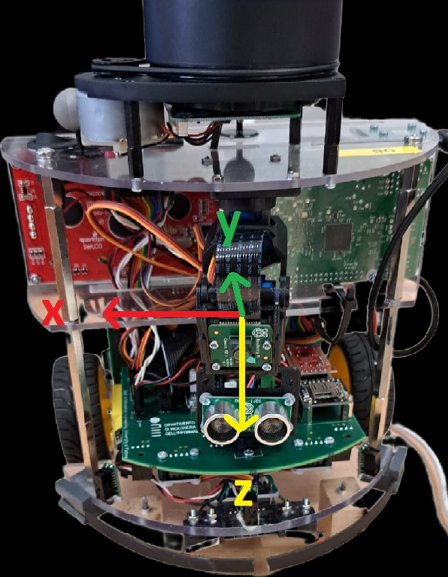
\includegraphics[width=0.50\textwidth, height=0.4\textheight]{figures/Lab2_1.png}
     \caption{The axis of the accelerometer}
     \label{fig:acc}
 \end{figure}
 \begin{itemize}
    \item \textbf{Tilt} refers to the vertical movement 
    of the camera, where the camera is moved up or down.
    \item \textbf{Pan} refers to the horizontal movement of the 
    camera, where the camera is rotated around its vertical axis
     to the left or right. 
 \end{itemize}
\subsubsection{Servo Motor}
A servo motor is a type of motor that is widely used in various 
applications, particularly in robotics, automation, and control systems.
It is designed to provide precise control over angular or rotational
movement. \newline

The distinguishing feature of a servo motor is its ability to maintain
 a specific position or follow a desired trajectory with great accuracy.
It achieves this through a closed-loop control system, which continuously
compares the actual position of the motor shaft with the desired position
and adjusts the motor's output accordingly. 

Here are some key components and characteristics of servo motors: 
\begin{itemize}
    \item \textbf{DC Motor}: Most servo motors are based on a DC motor
     as the primary driving mechanism. The DC motor converts electrical 
     energy into rotational motion. 
     \item \textbf{Gear Train}: Servo motors often include a gear train
      that reduces the motor's high-speed, low-torque output to a lower
       speed with higher torque. This gearing mechanism enables the servo
      motor to generate more precise and controlled movements.
    \item \textbf{Position Feedback Sensor}: A servo motor typically 
    incorporates a position feedback sensor, such as an encoder or a
     potentiometer. This sensor provides information about the current 
     position and velocity of the motor shaft. The feedback data is used
      by the control system to determine if the motor needs to adjust its 
    position.
    \item \textbf{Control Circuitry}: The control circuitry of a servo motor
     includes a microcontroller or a dedicated servo controller.
      It receives the control signal or command from an external device,
       such as a microcontroller or a computer, and generates the appropriate
        electrical signals to drive the motor. 
    \item \textbf{Pulse Width Modulation (PWM) Signal}: Servo motors commonly 
    utilize a PWM signal to control their position and speed. The control signal
     consists of a series of pulses with varying widths, where the width of each 
     pulse determines the desired position. The control circuitry interprets the
      pulse width and adjusts the motor's position accordingly. Figure (\ref{fig:PWM})
\end{itemize}
\begin{figure}[!h]
    \centering
    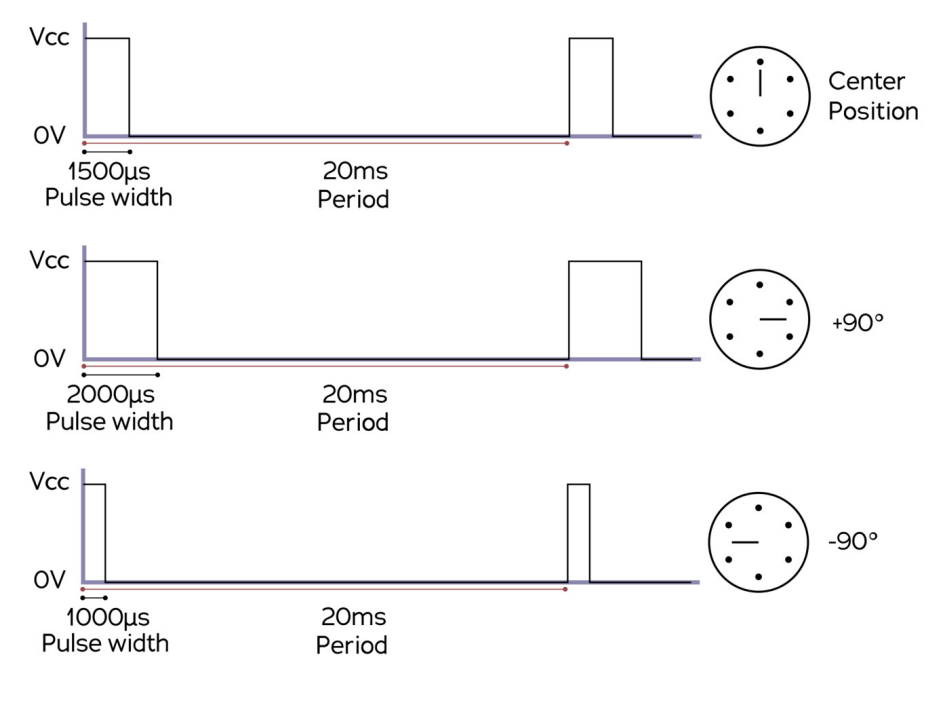
\includegraphics[width=0.80\textwidth, height=0.35\textheight]{figures/PWM.png}
    \caption{PWM signal and comtroling the position of the motor}
    \label{fig:PWM}
\end{figure}
\newpage
On the TurtleBot there are two servos that control the tilt and pan of the camera,
as shown in Figure (\ref{fig:motor}).
\begin{figure}[!h]
    \centering
    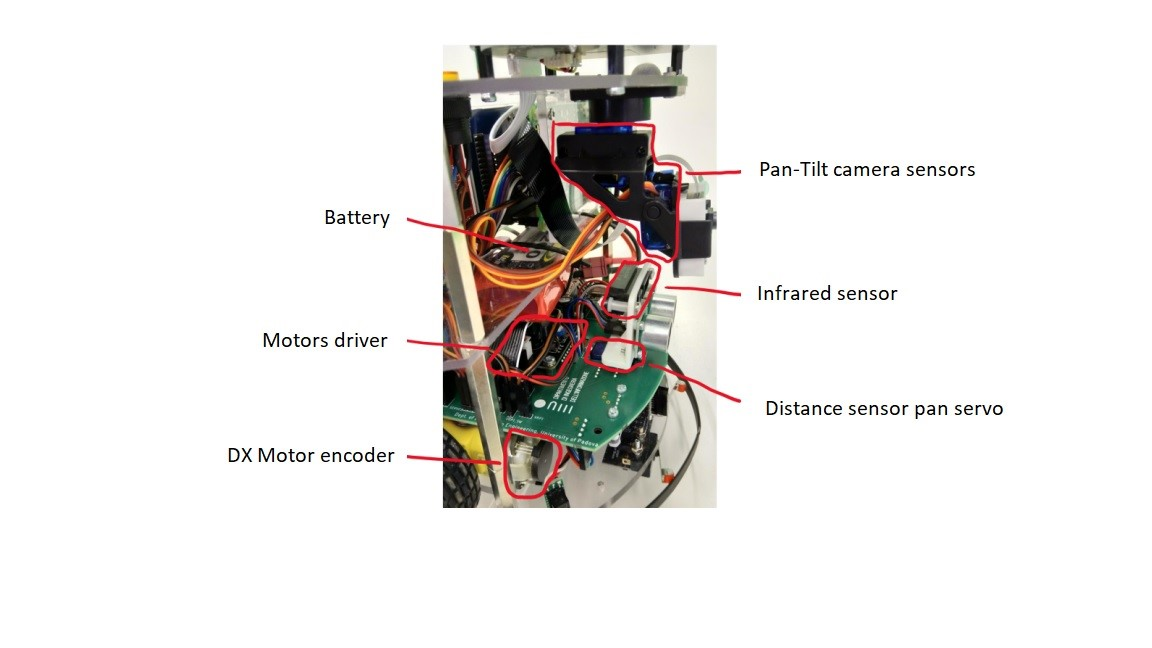
\includegraphics[width=1.10\textwidth, height=0.35\textheight]{figures/motor.png}
    \caption{PWM signal and comtroling the position of the motor}
    \label{fig:motor}
\end{figure}
\subsection{Exercises}
\subsubsection{Exercise1:}
Develop a control law to stabilize the camera’s tilt by utilizing data from an IMU. \newline
First of all, we have to keep the camera aligned (0 degree) with the horizon. For
this purpose, we should obtain the accelerometer and gyroscope data from the robot.
\begin{lstlisting}[language=C, caption={C code using listings}, label={lst:cameraTilt} ]

    int8_t tilt = 0; 
    float angle = 0; 
while (1) { 

    HAL_Delay(20); 
    bno055_convert_double_accel_xyz_msq(&d_accel_xyz); 
    angle = (asin(d_accel_xyz.y/ 9.81)) * 180 / 3.14; 
    tilt = -angle; 
    logger_data.u1 = tilt; 
    logger_data.u2 = d_accel_xyz.y; 
    ertc_dlog_send(&logger, &logger_data, sizeof(logger_data)); 
    ertc_dlog_update(&logger); 

    __HAL_TIM_SET_COMPARE(&htim1,
        TIM_CHANNEL_3,
        (uint32_t)saturate((150+tilt*(50.0/5.0)),
         SERVO_MIN_VALUE, 
         SERVO_MAX_VALUE));  

   } 
\end{lstlisting}
As you see, first we defined tilt and angle globally. 
To obtain the accelerometer data we use “bno055\_convert\_double
\_accel\_xyz\_msq”
and “d\_accel\_xyz” as a pointer to a structure as input.
\newpage
The formula for calculating the tilt angle of the TurtleBot is: 
\textbf{$\theta = \sin^{-1}\left(\frac{a_y}{g}\right)$} , $\theta$ is the tilt angle,
${a_y}$ is the acceleration measured on the y axis and g is gravity acceleration g = 9.81 $\frac{m}{s^{2}}$.
To convert $\theta$ from radiant the equation should be multiplied by $\frac{180}{\pi}$.
As we want to keep the camera aligned the tilt angle of the camera needs to be equal to -$\theta$ .\newline
For moving the camera the “\_\_HAL\_TIM\_SET\_COMPARE” is used. It is a HAL library macro
 used for setting the compare value of a specific channel of a hardware timer on the microcontroller. \newline

  To record sensor values a data logger is used. For this a structure is defined, which takes the necessary values. 
\begin{lstlisting}[language=C, caption={}, label={lst:datalog} ]
struct ertc_dlog logger; 

struct datalog { 
    float u1, u2; 
} logger_data;  
\end{lstlisting} 

Then we use logger\_data.u1 as the tilt data and logger\_data.u2 as the acceleration
measured on the y axis data in the while loop. 
\newline

To plot the\ data we use Matlab and the serial datalogger is invoked using serial\_datalog()
 function as below: 
\begin{lstlisting}[language=Matlab, caption={}, label={lst:serialDatalog} ]
data = serial_datalog('COM9',{'2*single','2*single'}, 'baudrate', 115200)
\end{lstlisting}
“COM9” is the port of the serial datalogger. “single,single” specifies the data 
format to be logged. It indicates that two data values will be logged in each 
iteration of the logging process. In this case, the logged data is expected to be
of type single (a single-precision floating-point number).\newline  
“baudrate”, “115200” sets the baud rate of the serial communication. 
The baud rate determines the speed at which data is transferred over the serial port.
 In this case, the baud rate is set to 115200 bits per second. 

\subsubsection{Bonus:}
Implement a control algorithm that implement a “smooth pan” control
(i.e. a control system that compensate sharp horizontal rotations of the TBot) 
using data from the gyroscope.\newline
Process is like exercise 1:

\begin{lstlisting}[language=C, caption={}, label={lst:smoothPan} ]
    int8_t pan = 0; 

    float angle = 0; 
while (1) { 
    HAL_Delay(20); 
    bno055_convert_double_gyro_xyz_rps(&d_gyro_xyz);
    angle = d_gyro_xyz.z * 180 / 3.14;
    pan = -angle/8;
    logger_data.u1 = pan; 
    logger_data.u2 = d_gyro_xyz.z; 
    ertc_dlog_send(&logger, &logger_data, sizeof(logger_data)); 
    ertc_dlog_update(&logger); 
    __HAL_TIM_SET_COMPARE(&htim1,TIM_CHANNEL_3,
    (uint32_t)saturate((150+pan*(50.0/55.0)),
     SERVO_MIN_VALUE,
    SERVO_MAX_VALUE));   
} 
\end{lstlisting}
 To compensate the pan motion of the camera the gyroscope angle around the z axis is measured. converted to degrees and negated the angle can be feed directly to the servo controlling for the pan motion. The result is a camera, which moves very jerky in the opposite direction of the TurleBots pan angle. To degrees the jerk of this motions a fraction of $\frac{1}{8}$ is used. The servo motor is set on “TIM\_CHANNEL\_3”.
\begin{figure}[tbh]
    \centering
    \includesvg[width=0.95\textwidth, height=0.9\textheight]{figures/plot.svg}
    \caption{Data captured while tilting and panning the TurtleBot}
    \label{fig:datal2}
\end{figure}

\clearpage

\section{Laboratory 3: Motor Control}
\subsection{Description}
The goal of this laboratory is to implement a controller to drive and 
control the DC motors of the TurtleBot. To reach that goal a PI controller is designed. The current angular speed is measured through an encoder on the motors. The reference input for the controller is angular speed , measured in rotation's per minute [rpm].
\subsubsection{DC Motor}
A DC motor is a class of rotary electrical motor that converts direct current (DC)
electrical energy into mechanical energy. There are three common parts in all types
of DC motors: 
\begin{itemize}
    \item a stator, which can be implemented as a permanent magnet; 
    \item a rotor winding or a coil, which can be simply a wire; 
    \item a commutator is connected to the rotor winding and its purpose is to force 
    the direction of the current flowing into the rotor to be always the same; 
\end{itemize}
However, the DC motor which is used in the Turtle-Bot uses Brushed implementation.
Brushes are used to feed current to the commutator and each brush is connected to
one pole of the power supply. 
\newpage
\begin{figure}[!h]
    \centering
    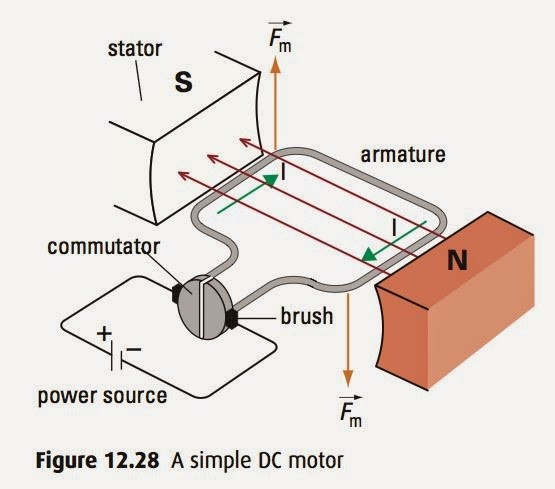
\includegraphics[width=0.60\textwidth, height=0.30\textheight]{figures/motorfig.png}
    \caption{DC Motor simplified scheme }
    \label{fig:motorfig}
\end{figure}
The stator generates a magnetic field and the rotor winding, which is positioned within
 the field generated by the stator, when a current flow through it, is subjected to a 
 magnetic force perpendicular to the direction of the stator field. The commutator has
  a ring-like shape and present gaps, so that each part of the commutator is connected
to power source of opposite polarity, ensuring the current flows in the proper
   direction. 

Inverting the power source polarity, invert the direction of the current, allowing 
the motor to rotate in both directions. 
\subsubsection{DRV8871}
Since we want to use a PWM as a control signal for the motor, we use a chip that can 
convert a PWM input into a proper output, both in terms of voltage and current, to 
drive the motor. For such purpose, the chosen chip is a DRV8871, which is a brushed
DC motor driver. The motor can be controlled bidirectionally by implementing an
H-bridge. 
\begin{figure}[!h]
    \centering
    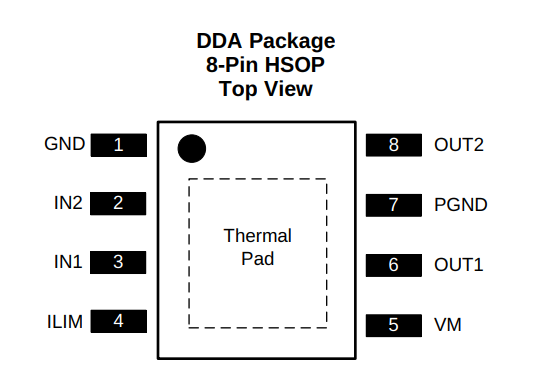
\includegraphics[width=0.60\textwidth, height=0.30\textheight]{figures/DRV.png}
    \caption{DRV8871 pinout}
    \label{fig:drv}
\end{figure}
\newpage
Below a description of some pins important to our case can be found. \newline
\begin{center}    
    \begin{tabular}{lS[table-format=3]cS[table-format=2.2]}
        \toprule
        \textbf{Pin Name} & \textbf{Pin Number} & \textbf{Pin Type} & \textbf{Description} \\
        \midrule
        IN1 & 3 & Input & \parbox{5cm}{Input of the chips that allow to control the output of the h-bridge. These pins receive the PWM signal from the microcontroller.}  \\ \\
        IN2 & 2 & Input & " "\\ \\
        OUT1 & 6 & Output & \parbox{5cm}{H-bridge output that goes to the motor}  \\ \\
        OUT2 & 8 & Output & " " \\
        \bottomrule
    \end{tabular}
\end{center}
The table below describes how the input signals can be used to control the output. 
\begin{center}
    \begin{tabular}{lS[table-format=3]cS[table-format=2.2]S[table-format=1.2]}
        \toprule
        Mode Name & {IN1} & IN2 & {OUT1} & {OUT2} \\
        \midrule
        Coast & 0 & 0 & Hi z & Hi z \\
        Reverse & 0 & 1 & L & H \\
        Forward & 1 & 0 & H & L \\
        Brake & 1 & 1 & L & L \\
        \bottomrule
    \end{tabular}
\end{center}
Coast mode allows the motor to coast to a stop, which means that the motor is not
 driven and will move by inertia. On the other hand, Brake mode will stop the motor
  faster. When used to drive the motor with PWM control signal with a duty
   cycle < 100\% and, for example, in forward mode, it is possible to alternate between
forward and brake mode or between forward and coast mode. 
\begin{figure}[!h]
    \centering
    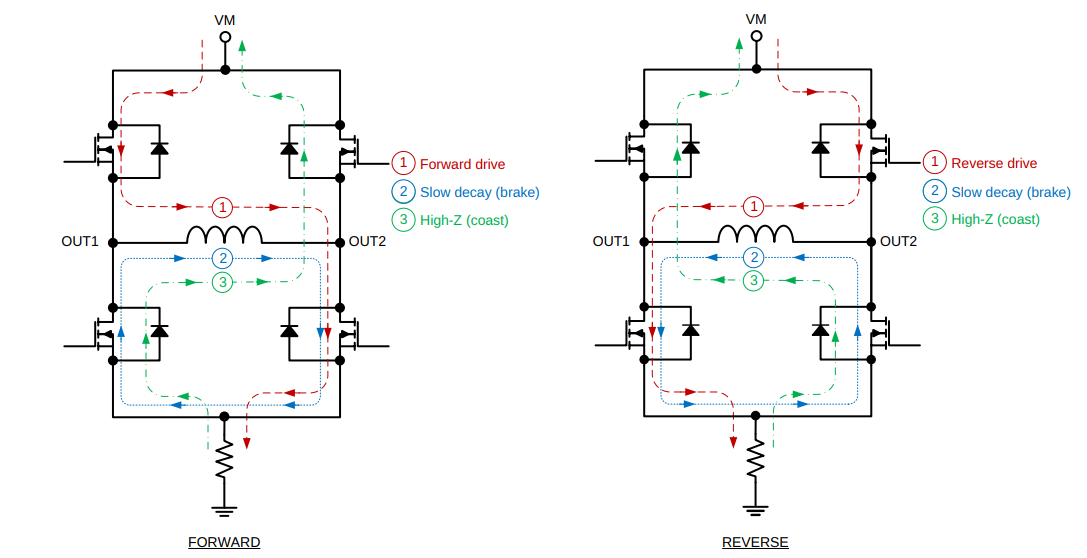
\includegraphics[width=0.90\textwidth, height=0.40\textheight]{figures/HBrige.png}
    \caption{H-Bridge Current Paths}
    \label{fig:bridge}
\end{figure}
\newpage
\subsubsection{PWM Setting}
The voltages applied to the inputs should have at least 800[ns] of pulse width 
to ensure detection. If the PWM frequency is 200[kHz], the usable duty cycle range 
is 16\% to 84\%.
\subsubsection{Position Encoder}
The position encoder is a sensor that transform a position information into an 
electrical signal. A quadrature encoder employs two outputs A and B which are called 
quadrature outputs, as they are 90 degrees out of phase; the direction of the motor 
depends on which phase’s signal lead over the other;  
\begin{figure}[!h]
    \centering
    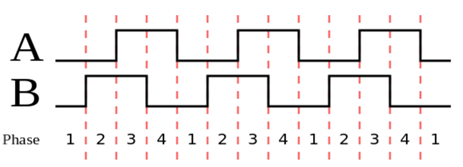
\includegraphics[width=0.70\textwidth, height=0.20\textheight]{figures/Encoder.png}
    \caption{Signals generated by a quadrature encoder with B leading over A }
    \label{fig:Enc}
\end{figure} \newline 
A counter can be used to measure the number of pulses 
(a pulse can be counted when an edge happens). 
\subsubsection{PID Controller:}
PID (Proportional Integral Derivative) controllers use a control loop feedback 
mechanism to control process variables and are the most accurate and stable controller.
\begin{figure}[!h]
    \centering
    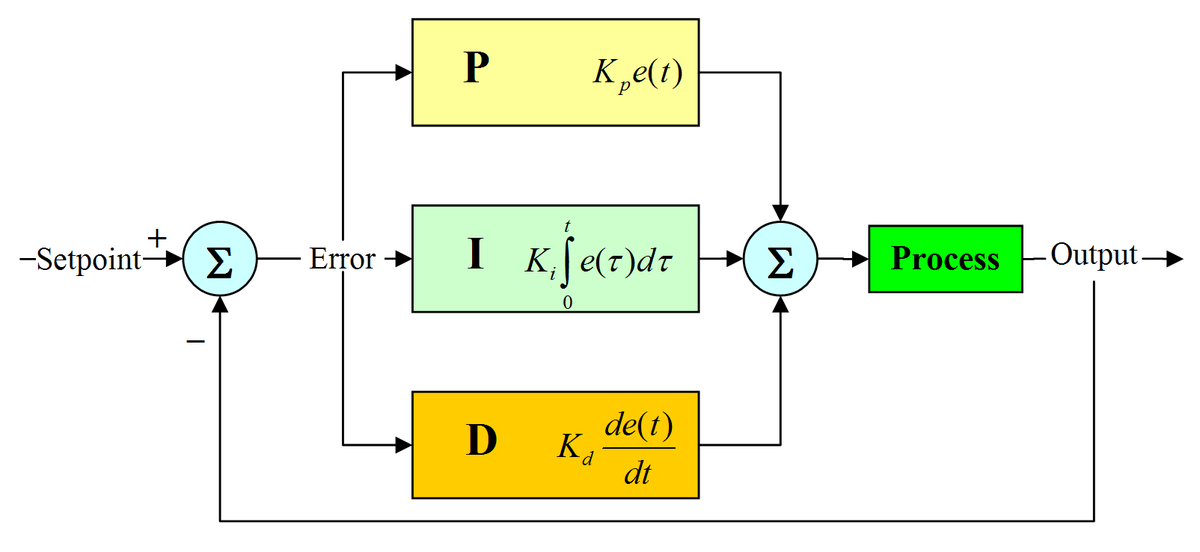
\includegraphics[width=0.80\textwidth, height=0.25\textheight]{figures/PID.png}
    \caption{PID Controller diagram }
    \label{fig:windup}
\end{figure}
Using the derivative control mode is a bad idea when the process variable has a lot
 of noise on it. 'Noise' is small, random, rapid changes in the process variable,
  and consequently rapid changes in the error. Because the derivative mode extrapolates
   the current slope of the error, it is highly affected by noise. Therefore, we only
    need to design and implement PI controller for this lab.
\subsubsection{Anti-Windup feature}
Integral windup refers to the situation in a PID controller where a large change in setpoint occurs (say a positive change) and the integral term accumulates a significant error during the rise (windup), thus overshooting and continuing to increase as this accumulated error is unwound (offset by errors in the other direction). The specific problem is the excess overshooting. 

Integral windup can come from derivative action or a large reference. In case of the TurtleBot, since no derivative control mode is used in the controller, only the reference may cause the overshooting.  

In order to solve the problem, an Anti-windup architecture is necessary. It is basically a saturation over the control output of the integrator, that keeps the error caused by the integral term of the controller in a desired range.  This prevents accumulation of the error and consequently the overshooting. The figure below illustrates a common Anti-windup architecture. 
\begin{figure}[!h]
    \centering
    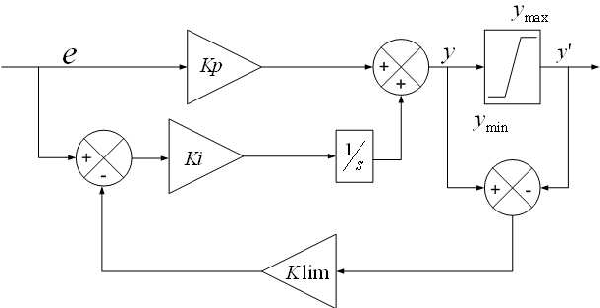
\includegraphics[width=0.80\textwidth, height=0.25\textheight]{figures/windup.png}
    \caption{Anti-windup architecture}
    \label{fig:pid}
\end{figure}
\subsection{Implementation details}
\subsubsection{Hardware setup and peripheral list}
\begin{itemize}
    \item TIM3 (16-bit, general-purpose timer), channel 1 and channel 2: Encoder for motor 1  
    \item TIM4 (16-bit, general-purpose timer), channel 1 and channel 2: Encoder for motor 2 
    \item TIM6 (16-bit, basic timer): Provide the clock for the controller 
    \item TIM8 (16-bit, advanced timer), channel 1 and channel 2: PWM for motor 1 
    \item TIM8 (16-bit, advanced timer), channel 3 and channel 4: PWM for motor 2 
\end{itemize}
\subsubsection{Motor and Encoder}
The module encompasses a gearbox with a 120:1 ratio, which means that for every round performed by the wheel, the motor rotates 120 times. 

The encoder provides 16 pulses per round. This means that the number of pulses per round from the wheel-side is 1920, assuming to use encoder mode 2X; this number is doubled when considering encoder mode 4X. Notice that this mode halves the quantization error, when compared with the 2X mode. 

The selected timer needs to be configured in encoder mode. Also, the counter period which can be setup to be equal to the number of pulses counted in one round (in this case 3840 since a 4X encoder mode is used) has to be taken into account. 
\begin{lstlisting}[language=C, caption={encoder code in order to have the current speed of each motor }, label={lst:encoder} ]
void HAL_TIM_PeriodElapsedCallback(TIM_HandleTypeDef *htim)
{
/* Speed ctrl routine */
if(htim->Instance == TIM6)
{
    uint32_t TIM3_CurrentCount , TIM4_CurrentCount;
            int32_t TIM3_DiffCount , TIM4_DiffCount;
            static uint32_t TIM3_PreviousCount = 0, TIM4_PreviousCount = 0;

        // read the counter value from the encoder
            TIM3_CurrentCount = __HAL_TIM_GET_COUNTER(&htim3);
            TIM4_CurrentCount = __HAL_TIM_GET_COUNTER(&htim4);

        //compute the difference between the current value and the old value
            /*  evaluate increment of TIM3 counter from previous count  */
            if (__HAL_TIM_IS_TIM_COUNTING_DOWN(&htim3)) // right motor
            {
                /* check for counter underflow */
                if (TIM3_CurrentCount <= TIM3_PreviousCount)
                    TIM3_DiffCount = TIM3_CurrentCount - TIM3_PreviousCount;
                else
                    TIM3_DiffCount = -((TIM3_ARR_VALUE+1) - TIM3_CurrentCount) 
                        - TIM3_PreviousCount;
            }
            else
            {
                /* check for counter overflow */
                if (TIM3_CurrentCount >= TIM3_PreviousCount)
                    TIM3_DiffCount = TIM3_CurrentCount - TIM3_PreviousCount;
                else
                    TIM3_DiffCount = ((TIM3_ARR_VALUE+1) - TIM3_PreviousCount) 
                        + TIM3_CurrentCount;
            }

            TIM3_PreviousCount = TIM3_CurrentCount;
            if (__HAL_TIM_IS_TIM_COUNTING_DOWN(&htim4)) // left motor
				{
					/* check for counter underflow */
					if (TIM4_CurrentCount <= TIM4_PreviousCount)
						TIM4_DiffCount = TIM4_CurrentCount - TIM4_PreviousCount;
					else
						TIM4_DiffCount = -((TIM4_ARR_VALUE+1) - TIM4_CurrentCount)
                             - TIM4_PreviousCount;
				}
				else
				{
				/* check for counter overflow */
					if (TIM4_CurrentCount >= TIM4_PreviousCount)
						TIM4_DiffCount = TIM4_CurrentCount - TIM4_PreviousCount;
					else
						TIM4_DiffCount = ((TIM4_ARR_VALUE+1) - TIM4_PreviousCount) 
                            + TIM4_CurrentCount;
				}

				TIM4_PreviousCount = TIM4_CurrentCount;
\end{lstlisting}
\subsubsection{PWM}
Configuration for the timer generating the PWM signal (TIM8): 
\begin{itemize}
    \item Clock source: APB1-Timer\_clocks at 96[MHz]; 
    \item Prescaler (PSC): 959 -> $f_T = 96 * (\frac{106}{96}) * 10 = 105 [Hz]$
    \item Counter period (Auto Reload Register): 399 -> $T_{PWM} = 4 * 102 * 10[s]$
\end{itemize}
\subsection{Exercises}
\subsubsection{Exercise1}
In order to control the DC motors, a PI Controller is used. 

By using the encoders (TIM3, TIM4), implemented in the way that has been explained 
in section 3.2.2, the number of pulses for each wheel is available. Considering 
that the counter period is the number of pulses per round from each wheel-side
 (in this case 3840 since a 4X encoder mode is used),  the 
 speed of the motors can be evaluate in round per minutes as follow: \newline
 \begin{center}
    $\textbf{speed[rpm]} = \frac{\textbf{number of pulses}}{\textbf{3840}} * \frac{60}{T_s}$
 \end{center}
 Which $T_s$ is the sampling time. Also the reference for the 
 speed of each motor in rpm is defined, which are hard coded. Therefore,  the tracking error can be 
 calculated, which will be considered as the input of
  the function PI\_controller. The output of the function is the control signal
   (in rpm) used to control the DC motors. 
\begin{lstlisting}[language=C, caption={calculating the control signal for DC motors in rpm }, label={lst:rpm} ]
// compute the motor speed in [rpm]
float current_rpm_R = ((float)TIM3_DiffCount/(2.0*1920.0))*(60.0/TS );
tracking_error_R = reference_rpm_R - current_rpm_R;

float current_rpm_L = ((float)TIM4_DiffCount/(2.0*1920.0))*(60.0/TS );
tracking_error_L = reference_rpm_L - current_rpm_L;

// compute the tracking error via PI controller
controller_return_R = PI_controller(tracking_error_R);
controller_return_L = PI_controller(tracking_error_L);

motor_V_R = controller_return_R;
motor_V_L = controller_return_L; 
\end{lstlisting}
A closed loop is established according to the following logic: 
The input of the function PI\_controller is the tracking error.
 The error signal is multiplied in parallel by two parameters, the 
 first is proportional gain $K_P$ producing the proportional term, and
  the second is the product of integral gain $K_I$ and the sampling period 
   $T_s$, producing the integral term.  

To avoid overshooting in the response, caused by accumulation of the 
integrator error, an Anti-windup scheme is set up. It is a saturation over
$E_I$. The threshold of the error which is 10 has been selected by trial and error.
The optimal values of the $K_P$  and $K_I$ are found by trial and error. 
\begin{lstlisting}[language=C, caption={PI Controller}, label={lst:PI} ]
float Kp = 0.34;
float KI = 0.2;

float PI_controller (float error){
    float P = Kp * error;
    static float I = 0;
    I = I + error * KI * TS;
    if(I>10){ // anti windup
        I=10;
    }
    return P + I;
}    
\end{lstlisting}
After summing up the proportional and integral term and producing the output
 of the function (control signal in rpm), it will be fed to the DC motors
  through TIM8 as PWM signals. Notice that TIM6 is acting as a clock in the
   system. All the steps needed to accomplish the goal, should be executed 
   from inside the HAL\_TIM\_PeriodElapsedCallback function, which is a callback
    function called when a timer’s period is elapsed. 

    A linear relationship between the duty cycle and
     the voltage applied to the motor is assumed. The supply voltage $[o, V_{PowerSupply}]$. $V_{PowerSupply}$ ,depending on the power supply source,
    is assumed equal to $V_{BAT} = 8[v]$.
\newpage
\begin{lstlisting}[language=C, caption={calculating duty cycle}, label={lst:duty} ]
#define VBATT	8.0 
#define V2DUTY	((float)(TIM8_ARR_VALUE+1)/VBATT) 
#define DUTY2V	((float)VBATT/(TIM8_ARR_VALUE+1)) 

// calculate duty cycle for motor 

int32_t duty_R = V2DUTY*motor_V_R; 

int32_t duty_L = V2DUTY*motor_V_L;   
\end{lstlisting}
According to the Counter Period of TIM6, generating the PWM signal,
a saturation of 399 is set over each duty cycle to prevent over driving the motors. 
\begin{lstlisting}[language=C, caption={calculating duty cycle and command the motors}, label={lst:duty1} ]
// calculate duty cycle for motor
int32_t duty_R = V2DUTY*motor_V_R;
int32_t duty_L = V2DUTY*motor_V_L;

if (duty_R > 399)
duty_R = 399;

/* calculate duty properly */
if (duty_R >= 0) { // rotate forward
    // alternate between forward and coast
    //__HAL_TIM_SET_COMPARE(&htim8, TIM_CHANNEL_1, (uint32_t)duty_R);
    //__HAL_TIM_SET_COMPARE(&htim8, TIM_CHANNEL_2, 0);

    // alternate between forward and brake, TIM8_ARR_VALUE is a define
    __HAL_TIM_SET_COMPARE(&htim8, TIM_CHANNEL_1,
         (uint32_t)TIM8_ARR_VALUE);
    __HAL_TIM_SET_COMPARE(&htim8, TIM_CHANNEL_2,
         (uint32_t)(TIM8_ARR_VALUE - duty_R));
} else { // rotate backward
    __HAL_TIM_SET_COMPARE(&htim8, TIM_CHANNEL_1, 0);
    __HAL_TIM_SET_COMPARE(&htim8, TIM_CHANNEL_2, (uint32_t)-duty_R);
}

if (duty_L > 399)
    duty_L = 399;

/* calculate duty properly */
if (duty_L >= 0) { // rotate forward
    // alternate between forward and coast
    //__HAL_TIM_SET_COMPARE(&htim8, TIM_CHANNEL_3, (uint32_t)duty_L);
//__HAL_TIM_SET_COMPARE(&htim8, TIM_CHANNEL_4, 0);

    // alternate between forward and brake, TIM8_ARR_VALUE is a define
    __HAL_TIM_SET_COMPARE(&htim8, TIM_CHANNEL_3,
         (uint32_t)TIM8_ARR_VALUE);
    __HAL_TIM_SET_COMPARE(&htim8, TIM_CHANNEL_4, 
         (uint32_t)(TIM8_ARR_VALUE - duty_L));
} else { // rotate backward
    __HAL_TIM_SET_COMPARE(&htim8, TIM_CHANNEL_3, 0);
    __HAL_TIM_SET_COMPARE(&htim8, TIM_CHANNEL_4, (uint32_t)-duty_L);
} 
\end{lstlisting}
\newpage
Since the control is implemented using the Forward/Break 
technique in Exercise 1, the commands to the motors are setup in
 the way that is shown in Listing \ref{lst:duty1}  To collect the sensor values the data logger is setup to save and plot all relevant information.
   The set up is as follows: 
\begin{lstlisting}[language=C, caption={setting up data logger}, label={lst:date} ]
data.w1 = reference_rpm_R;
data.w2 = current_rpm_R;
data.u1 = tracking_error_R;
data.u2 = controller_return_R;


data.x1 = reference_rpm_L;
data.x2 = current_rpm_L;
data.y1 = tracking_error_L;
data.y2 = controller_return_L;

ertc_dlog_send(&logger, &data, sizeof(data));  
\end{lstlisting}
The results are plotted as shown below:
\begin{figure}[tbh]
    \centering
    \includesvg[width = 1.5\textwidth, height=0.6\textheight]{figures/LAB3_forwardandbreak_with_antiWindup_2.svg}
    \caption{The results of the control using the Forward/Brake technique}
    \label{fig:b2}
\end{figure}
\newpage
To conclude, the results show that after turning on the motors, 
it takes a few milliseconds for motors to reach desired speed 
(acceptable rise time); even after being turned off for a while,
 the over-shoot does not go higher than a certain and reasonable
  level of speed (effect of the Anti-windup scheme). Lastly, the
   step response is settled at the reference value in few seconds.
    Notice that the noise in the response is because of the nature of
    the system and the digital controller. 
\subsubsection{Exercise2}
In order to implement the controller with the Forward/Coast 
technique,  the alternative piece of code is changed,
 shown in Listing \ref{lst:duty1}. 
 \begin{figure}[tbh]
    \centering
    \includesvg[width = 1.5\textwidth, height=0.6\textheight]{figures/LAB3_forwardandcoast_with_antiWindup_2.svg}
    \caption{The results of the control using the Forward/Coast technique }
    \label{fig:b3}
\end{figure}\newline
Coast mode allows the motor to coast to a stop, which means that the motor 
is not driven and will move by inertia. On the other hand, brake mode will 
stop the motor faster. Therefore, the step response of motor implemented by
Forward/Coast technique has more noises (even when the motor is set to be off)
which can be interpreted as the inertia.  
\subsubsection{Exercise Bonus}
The Anti-windup is implemented in the way that has been explained in
section 3.3.1, particularly in Listing \ref{lst:PI}. As mentioned before the
threshold for the saturation has been chosen by trial and error. 
However, the first Anti-windup method used was to set directly a 
saturation over the voltages fed to the motors. After saturating the
voltage directly by changing the threshold to different values 
(for example, 4 in Listing \ref{lst:anti}), the overshoot problem was still unsolved. 
Hence,  the Anti-windup method had to saturate only the
 integral term of the control signal, shown 
 in Listing \ref{lst:PI}. 
\begin{lstlisting}[language=C, caption={wrong Anti-windup method}, label={lst:anti} ]
if(motor_V_R > 4)
    motor_V_R = 4;
if(motor_V_R < -4)
    motor_V_R = -4;

if(motor_V_L > 4)
    motor_V_L = 4;
if(motor_V_L < -4)
    motor_V_L = -4;
\end{lstlisting}
The step response of the motors using both Forward/Break and
Forward/Coast techniques, when the Anti-windup implementation
is not used are shown in Figure \ref{fig:b4} and Figure \ref{fig:b5}. To conclude, 
the step response of the system (no matter implemented by which technique),
 without implementing an Anti-windup feature, has a large overshoot due
  to the accumulation of the error caused by integral term. Adding an 
  Anti-windup feature enhances the overall performance and reduced the 
  overshoot in the system, as expected (Figure \ref{fig:b2} and Figure \ref{fig:b3}).
\begin{figure}[tbh]
    \centering
    \includesvg[width = 1.5\textwidth, height=0.6\textheight]{figures/LAB3_forwardandbreak_with_NOantiWindup.svg}
    \caption{The results of the control using the Forward/Break technique without Anti-windup} 
    \label{fig:b4}
\end{figure} 
\newpage
\begin{figure}[tbh]
    \centering
    \includesvg[width = 1.5\textwidth, height=0.6\textheight]{figures/LAB3_forwardandcoast_with_NOantiWindup.svg}
    \caption{The results of the control using the Forward/Coast technique without Anti-windup} 
    \label{fig:b5}
\end{figure} 

\newpage
\section{Laboratory 4: Line Following}
\subsection{Description}
The goal of this laboratory was to combine the line sensor from
Lab 1 and the motor controller from Lab 3 to make the TurtleBot 
follow a given line autonomously.  

\subsubsection{The infrared line sensor} 
A Pololu QTR reflectance sensor is used, which can detect how much infrared 
light has been reflected from a surface. With a certain threshold the difference between dark and light surfaces can be determent. The installed sensor is located on the lower front of the
 robot. It is about 10 cm wide and consists of an array of 8 photo diodes with each one 
 photo transistor. The distance between every sensor is 8 mm. This gives a total of 8
  individual sensors that can differentiate between dark and light areas. This data is 
 retrieved by the controller MCU through a port expander board using a I2C connection.
  The sensor data encoded in a binary format and received as an integer. To retrieve
  the original data, it is necessary to convert the integer back to a binary number.
 This binary number has 8 bits, each storing the value of one sensor.  
 
\subsubsection{Properties of the line} 
The line is assumed to be wide enough to trigger at least one of the infrared sensors 
and at most two at the same time. The goal is to create a controller algorithm that 
keeps the line between the two middle sensors 3 and 4. A tracking 
error is implemented and center position is defined as tracking error 0. The tracking error is defined to be greater than zero when the line is on the left side of the sensor. If the tracking 
error is less than zero, the line is on the right side of the sensor. Figure \ref{fig:line}
\begin{figure}[!h]
    \centering
    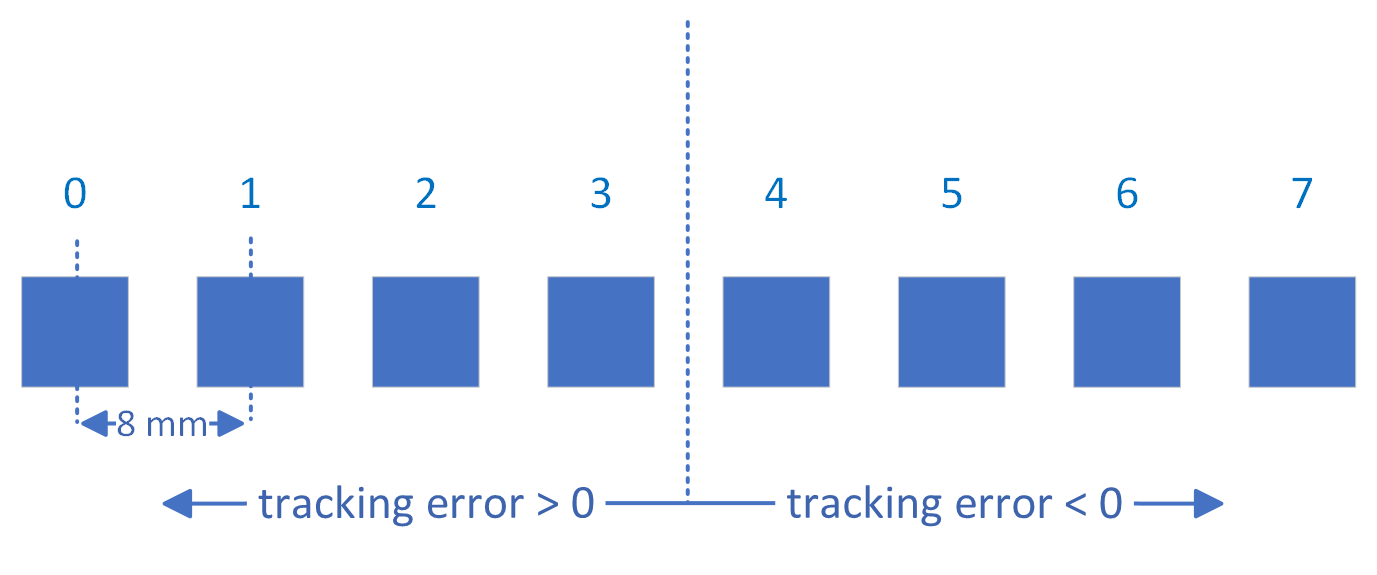
\includegraphics[width=0.90\textwidth, height=0.25\textheight]{figures/line.png}
    \caption{Spacing of the infrared sensors}
    \label{fig:line}
\end{figure}

\begin{figure}[!h]
    \centering
    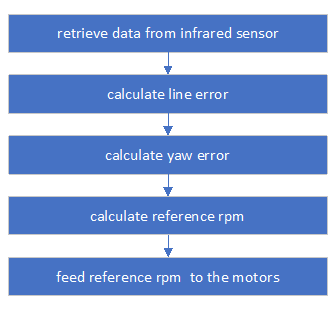
\includegraphics[width=0.45\textwidth, height=0.25\textheight]{figures/procedure.png}
    \caption{Main structure of the line following code}
    \label{fig:pro}
\end{figure}
\newpage
In LAB1 a function was already created to get the binary values of the integer received by the line sensor. However, this function would output an integer again,
  with all the bits in a single number. This was not a very useful implementation.
  It was necessary to get the bits in an array. For that an empty array is defined in the callback
 function (Listing \ref{lst:callback}) and the pointer is given to the findBinary function. The basic
 decimal to binary converter in form of a while function would then store every bit in
  this array, Listing \ref{lst:binary}.
\begin{lstlisting}[language=C, caption={converts integer to a binary array}, label={lst:binary} ]
void findBinary(int decimal, int * binary){
    int i =0;
    while(decimal > 0){
        int rem = decimal % 2;
        binary[i] = rem;
        i++;
        decimal = decimal / 2;
       }
}
\end{lstlisting}
\begin{lstlisting}[language=C, caption={Top part of the timer callback function }, label={lst:callback} ]
    void HAL_TIM_PeriodElapsedCallback(TIM_HandleTypeDef *htim)
{
	/* Speed ctrl routine */
	if(htim->Instance == TIM6) // check if interrupt came from timer
	{
		// get the line sensor data
		status = HAL_I2C_Mem_Read(&hi2c1,
                    SX1509_I2C_ADDR1 << 1,
                    REG_DATA_B, 1,
                    &lineData, 1,
                    I2C_TIMEOUT);
    int binary[8] = {0};
    findBinary(lineData, binary); // converts int to binary array
    
\end{lstlisting}
The calc\_error\_line function shown in Listing \ref{lst:calcer} does the calculation of the 
line error. The input of this function is an 8-dimensional array, containing
the state of each infrared sensor coded in binary. A logical one means, that
the corresponding sensor has detected a dark spot. The for loop iterates
through every value in the binary[] array, ergo through all sensors data. The sum of the binary[] array is calculated to get the total number of triggered 
sensors. Furthermore,  the "distance\_from\_middle" array is filled with the 
 opposing distance of every sensor from the middle. The distance between every
 sensor is 4mm. These values get negative to indicate a distance to the left and 
positive to indicate a distance to the right. The sum\_dist value is the sum of
every distance from the center if the sensor was activated. Calculating the 
line\_error by dividing the sum of the distance of each activated sensor with
 the total number of activated sensors. This line\_error represents the 
 offset of the black line from the center, regardless of how wide the line is.
  Even if only one sensor is not activated, a useful line error value is calculated. 
\begin{lstlisting}[language=C, caption={Function to calculate the line error based on a binary array }, label={lst:calcer} ]
int calc_error_line (int binary[]){
    float distance_from_middle[8]={0};
    float sum_dist = 0;
    int sum_binary = 0;
    for(int n=0;n<8;n++){
        sum_binary += binary[n];
        distance_from_middle[n]=((7.0/2.0)-n)*4;
        sum_dist += binary[n]*distance_from_middle[n];
    }
    float line_error = sum_dist / sum_binary;
    return line_error;
}
\end{lstlisting}
\newpage
\begin{lstlisting}[language=C, caption={Conversion from line error to yaw error }, label={lst:yaw} ]
float calc_yaw_error(float line_error){
    float phi_err = line_error/85;
    float yaw_err = phi_err * (165/2);
    return yaw_err;
}
\end{lstlisting}
The calc\_yaw\_error function in Listing \ref{lst:yaw} calculates a much stabler result
 for the error value. It includes the wheelbase dimension (D) and the 
 distance between the line sensor and wheels (H). This determines the 
 position of the turning point of the bot, which is between the two wheels, 
 shown in Figure (\ref{fig:turt}) 
 \begin{figure}[!h]
    \centering
    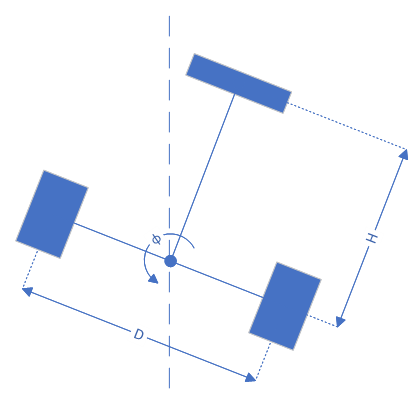
\includegraphics[width=0.55\textwidth, height=0.35\textheight]{figures/tut.png}
    \caption{Schematic of the wheelbase and line sensor placement\newline 
    D=165 mm, H=85 mm}
    \label{fig:turt}
\end{figure}
\subsubsection{Calculating the reference for the motors}

Based on the yaw error the reference for the two motors is calculated.
Since the motor controller is designed to compute rotations per minute, a base speed of 100 rpm is set and depending on the direction of the motor the yaw error add or subtract. To give the yaw error more effect on the base speed, an additional gain is incorporated. Testing different gains, a reliable solution with
a base speed of 100 rpm +- yaw\_error * 12 was found. By Increasing the gain, the performance in sharper corners got better. The drawback was increased instability
 on the straight segments. Small changes in the yaw error multiplied with 
 a high gain gave the bot a very shaky ride in straight segments. To furthermore 
 improve the performance a linear or even an exponential gain was necessary. 
 This would increase the impact of the yaw error in tighter corners and make 
 sure to decrease the gain when the line is going straight. The robot would 
 be very stable on straight lines and keep its agile performance in sharp corners. 
 One solution was to implement different "if" statements to check if the yaw error was in
  a certain range. Then different gains could be set accordingly. This worked, 
  but needed a lot of tuning of all the values. The settled values for each section of the if statements where very similar to the yaw error itself.   
 A very simple solution was to square the yaw error.
  This would increase the gain linearly. To keep the
   sign of the yaw error, the absolute value of the yaw 
   error was multiplied by itself, see Listing \ref{lst:refre}. For tuning
    this setup to use different base speeds it is possible to
     also add a gain to increase the impact of the squared yaw error.   
\begin{lstlisting}[language=C, caption={Calculating the reference signals for the motors}, label={lst:refre} ]
reference_rpm_L = 100 - yaw_err*ABS(yaw_err); // workes great 
reference_rpm_R = 100 + yaw_err*ABS(yaw_err);
\end{lstlisting}
\newpage
The plot of Figure \ref{fig:datal4} shows the signals of the left and right motor. There is also 
shown the line and yaw error calculated from the data collected by the line sensor.
The reference signal for each motor is then set by the functions shown in Listing \ref{lst:refre}.
It is clear to see that the encoder value of each motor is tracing the reference 
signal great. It is also clear to see the limitations of the motors. When the
reference exceeds a given speed of around 150 rpm, the motors are limited by the 
duty cycle implemented in LAB 3. The solution for this would be to set a limit to
the reference signal when calculated. Because of the geometry of the robot,
calculating the yaw error results in a very similar value of the line error.
This is because the ratio between wheelbase (D) to distance of line (H) sensor 
to wheels is almost one half, shown in Figure \ref{fig:turt}. 
\begin{figure}[tbh]
    \centering
    \includesvg[width=0.9\textwidth, height=0.8\textheight]{figures/plotLab4.svg}
    \caption{Motor Level Plot}
    \label{fig:datal4}
\end{figure}

\clearpage
\appendix

\section{Section in the Appendix}
\label{sec:app1}

\subsection{Subsection in the Appendix}
\label{subsec:app2}

Additional relevant information...

\end{document}
